\chapter{Teaching Your PI Controller to Behave (Part VI)}\label{ch:6}

I am writing this particular blog installment while lying by a swimming pool in a resort on the Riviera Maya.  There are lots of beautiful distractions which are competing for my attention, including my gorgeous 20 month old granddaughter who is playing at my feet.  So I have to disclaim any liability related to the quality of this particular blog!

So far in this series we have discussed how to set the coefficients for the PI controllers in a cascaded speed control loop.  We saw that $K_b$ is used for pole-zero cancellation within the current loop.  $K_c$ and Kd are indexed to the velocity feedback filter’s time constant, and are calculated by first selecting a suitable damping factor which is related to the responsiveness and damping of the system.  We also saw that $K_a$ sets the current controller’s bandwidth.  But what should that bandwidth be?

It turns out that we have two competing effects vying for control of where we set $K_a$.  On the bottom end of the frequency range, we have the velocity feedback filter pole with some really nice tan lines that wants to push the current controller pole to higher frequencies so as to not interfere with our nice tuning procedure.  But we can only go so high before we start running into other problems.  Let’s take a look at both ends of the frequency spectrum in an effort to understand these issues, and hopefully gain some insight into how to judiciously set $K_a$.  But first, let’s rewrite the open-loop transfer function of the velocity loop to once again include the current controller’s transfer function:

\begin{equation}\label{eq:6_1}
    gH(s) = \frac{K K_cK_d \left(1+\frac{s}{K_d}\right)}{s^2 \left(1+\frac{L}{K_a}s\right)\left(1+\tau s\right)}
\end{equation}

where
\begin{itemize}
    \item $K$ is a coefficient that contains several terms related to the motor and load
    \item $K_c$ and $K_d$ are the PI coefficients for the velocity loop
    \item $L$ is the motor inductance
    \item $K_a$ is one of the PI coefficients for the current loop
    \item $t$ is the time constant of the velocity feedback filter
    \item $s$ is the Laplace frequency variable
\end{itemize}

Our tuning procedure assumes that the current controller’s closed-loop gain is always unity, which implies it has infinite bandwidth.  But in reality, as long as the current controller’s bandwidth is at least 10x higher than the velocity loop unity gain frequency, our tuning procedure is still pretty good at predicting the system response.  If this condition isn’t satisfied, the current controller pole starts interfering with the velocity loop phase margin, resulting in a more underdamped response than our tuning procedure would otherwise indicate.

Figure \ref{fig:06_01} shows an example case to illustrate this point.  The {\color{SpringGreen4}green} curve represents what the tuning procedure predicts the normalized step response should be for a system with a damping factor of \num{2.5}.  The {\color{red}red} curve shows what happens when the current controller’s bandwidth is reduced to equal the velocity filter’s bandwidth.  The system is still stable, but the damping is much less than predicted from our tuning procedure.  At this point, we have two options\dots either increase the damping factor (and consequently lower the frequency response of the velocity loop), or increase the current loop bandwidth by increasing $K_a$.  The {\color{Cyan4}cyan} curve shows the first option where we increase the damping factor just enough to bring the overshoot down to the predicted value.  Unfortunately this increases the step response transient time as well.  The {\color{Gold2}yellow} curve shows the latter option where we put the damping factor back to \num{2.5}, and increase the current controller’s pole to be 10x higher than the velocity loop unity gain frequency.  As you can see, the actual response more closely resembles the predicted value.  The higher the current controller’s bandwidth is, the closer the response will resemble the predicted response.

\begin{figure}[H]
    \centering
    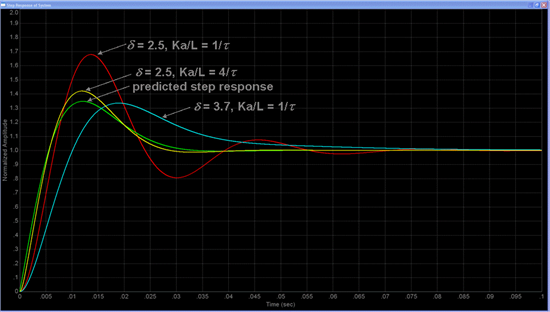
\includegraphics[width=1\linewidth]{06/01}
    \caption{Step Response of a System with Variable Damping and Pole Placement}
    \label{fig:06_01}
\end{figure}

So from this exercise, we might conclude that the best strategy is to set the current controller bandwidth to be as high as possible.  But is this really the best course of action?  As my dear ol’ grandma used to say, “Never use a 1 \unit{\giga\Hz} op-amp when a \qty{1}{\mega\Hz} op-amp will do the job.”  (Well, she never actually said it in those exact words, but you get the point).  Usually high bandwidth in \textit{any} system results in unruly and obnoxious behavior, and should only be used if absolutely necessary.  In this case, high current loop bandwidth often results in undue stress on your motor, since high frequency \textit{current} transients and noise translate into high frequency \textit{torque} transients and noise.  This can even manifest itself as \textit{audible} noise!  But there is also another limit on your current loop bandwidth:  the \textit{sampling frequency}.

Take a look at Figure \ref{fig:06_02} which shows a digital Field Oriented Control (FOC) based Variable Frequency Drive (VFD).  To simplify the discussion, we will assume that the entire control loop is clocked by a common sampling signal, although in real-world applications we often choose to sample the velocity loop at a much lower frequency than the current loop to save processor bandwidth.

\begin{figure}[H]
    \centering
    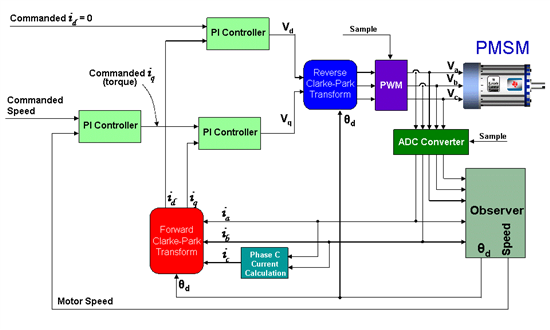
\includegraphics[width=1\linewidth]{06/02}
    \caption{Digital Field Oriented Control System for a PMSM.}
    \label{fig:06_02}
\end{figure}

In an analog system, any change in the motor feedback signals immediately starts having an effect on the output control voltages.  But with the digital control system of Figure \ref{fig:06_02}, the motor signals are sampled via the ADC at the beginning of the PWM cycle, the control calculations are performed, and the resulting control voltages are deposited into double-buffered PWM registers.  These values sit unused in the PWM registers until they are clocked to the PWM output at the start of the next PWM cycle.  From a system modeling perspective, this looks like a sample-and-hold function with a sampling frequency equal to the PWM update rate frequency.  The fixed time delay from the sample-and-hold shows up as a lagging phase angle which gets progressively worse at higher frequencies.  Figure \ref{fig:06_03} shows a normalized frequency plot of the phase delay for a sample-and-hold function, where the sampling frequency is assumed to be 1.  As you can see, the phase delay reaches down into frequencies much lower than the sampling frequency.  For example, at one decade below the sampling frequency, the S\&H is still affecting a phase shift of \qty{-18}{\degree}.

\begin{figure}[H]
    \centering
    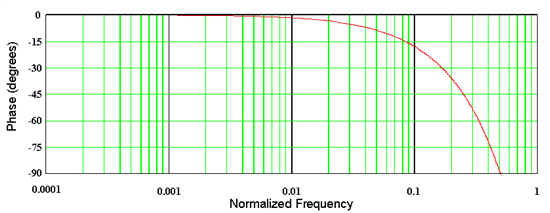
\includegraphics[width=1\linewidth]{06/03}
    \caption{Phase Lag Plot for a Sample-and-Hold, $F_s = 1$}
    \label{fig:06_03}
\end{figure}

Since the current controller processes higher bandwidth signals than the velocity loop, it is usually the current loop that suffers most by the S\&H effect of the PWM module.  Since the PWM S\&H is in series with the signal path for the current loop, its magnitude and phase contributions add directly to the open-loop response for the current controller.  If we rewrite the equation for the open-loop response of the current controller (assuming $K_b = R/L$), we end up with the following function:

\begin{equation} \label{eq:6_2}
    GH_c(s) = PI(s) \cdot \frac{I(s)}{V(s)} = \left(\frac{K_a}L\right)\left(\frac1s\right)
\end{equation}

This is simply an integrator function with gain of $K_a/L$.  Unity gain will obviously occur when $s = K_a/L$.  The single pole at $s = 0$ implies that the unity gain frequency will have a \qty{90}{\degree} phase shift, which also implies a \qty{90}{\degree} phase margin.  However, for a digital control system, you must add the phase lag shown in Figure \ref{fig:06_03}.  To do this, calculate for the following frequency ratio:

\begin{equation} \label{eq:6_3}
    \frac{K_a T_s}{2\pi L}\,\text{where $T_s$ is the sampling period}
\end{equation}

Then use Figure \ref{fig:06_03} to determine how much phase lag you must subtract off of your phase margin.  For example, if $K_aT_s/(2\pi L) = 0.1$, then you must subtract off \qty{18}{\degree} from your phase margin, leaving you with a comfortable \qty{72}{\degree}.  In most designs you probably want to keep $Ka/(2\pi L)$ at least an order of magnitude below the sampling frequency.  So using this assumption as well as the constraints from the velocity loop tuning procedure, we can now write a general “rule of thumb” expression for the range of $K_a$:

\begin{equation}\label{eq:6_4}
    \frac{10L}{\delta \tau} < K_a < \frac{\pi L}{5 T_s}
\end{equation}
where:
\begin{itemize}
    \item $L$ is the motor inductance
    \item $\tau$ is the time constant of the velocity filter
    \item $\delta$ is the damping factor
    \item $T_s$ is the sampling period
\end{itemize}


In most designs this still leaves a fairly broad range for the value of $K_a$.  In my experience, I have found that erring on the side of the current bandwidth being too low is usually better than being too high.  Snappy waveforms look nice on an oscilloscope, but your application may not need (or want) all that bandwidth.

Up until now, we have only dealt with “small signal” conditions (i.e., linear operation with no saturation effects).  But in the real world, step transient responses almost always saturate the system’s voltage or current levels, which tend to lengthen the response times.  When this happens, you can increase the PI gains all you want, but it won’t speed up the response.  In fact, it will usually just make the overshoot worse, since the integrator is acting on a gained-up error signal, which it will just have to dump eventually.  So how do we deal with this problem?  Are we doomed to simply using low integrator gains?  It turns out that there is another solution which doesn’t involve changing your integrator gains, which I will discuss in my next blog.  Until then\dots\\


Keep Those Motors Spinning,\\

\includegraphics[width=0.2\linewidth]{01/04_dave}
\vfill
\textit{Apr 04 2013 23:24 PM}